\subsection{Blochtheorie und Bändermodell}

Für die Rastertunnelmikroskopie ist die räumliche Verteilung der Elektronen an 
der Oberfläche von zentraler Bedeutung. Die Blochtheorie macht Aussagen über 
die Aufenthaltswahrscheinlichkeiten von Elektronen in periodischen 
Gittern und liefert ein Modell zur Erklärung des Bändermodells. 
Für ein Elektron mit Wellenfunktion $\psi$ gilt bei Vernachlässigung der 
Elektron-Elektron-Wechselwirkung in der nichtrelativistischen Näherung die 
Schrödingergleichung 
\begin{equation}
    \hat H \psi(\R) = \Big[ - \frac{\hbar^2}{2m} \Delta + V(\R) \Big] \psi(\R) = E \psi(\R)
\end{equation}
mit periodischem Potential
\begin{equation}
    V(\R) = V(\mathbf{r + r_n}); 
\qquad \mathbf{r_n} = n_1 \mathbf{a_1} + n_2 \mathbf{a_2} + n_3 \mathbf{a_3} 
\end{equation}
wobei $\mathbf{a_i}$ Gittervektoren des Ortsraumes sind. Auf Grund der Periodizität lässt 
sich das Potential in eine Fourierreihe zerlegen:
\begin{eqnarray}
    V(\R) &= &\sum_\G \VG \mathrm{e}^{i\G \cdot \R} \\
    \mathrm{mit \ Fourierkomponente \quad}  \VG &= &\frac{1}{L} \int \mathrm{e}^{i\G \cdot \R} 
    V(\R) \mathrm{d}\R  \nonumber \\
    \mathrm{und \ reziprokem \ Gittervektor \quad} \G &= &h\mathbf{g_1} + k\mathbf{g_2} +l\mathbf{g_3}; 
    \quad h, \ l, \ k, \ \in \mathbb{Z}. \nonumber
\end{eqnarray}

Der Ansatz für die Lösung ist eine Linearkombination ebener Wellen
$ \psi(\R) = \sum_\K C_\K \mathrm{e}^{i\K \cdot \R}, $
für die nach Einsetzen in die Schrödingergleichung gelten muss:
\begin{equation}
    \sum_\K \mathrm{e}^{i\K \cdot \R} 
    \Big[ \Big( \frac{\hbar^2 k^2}{2m} - E\Big) C_\K + \sum_\G \VG C_{\K - \G}\Big] 
    = 0
\end{equation}
Aus der Unabhängigkeit von $\R$ folgt dann
\begin{equation}
    \Big( \frac{\hbar^2 k^2}{2m} - E\Big) C_\K + \sum_\G \VG C_{\K - \G}= 0
\end{equation}

Zu jeden $\K$ Wert ergeben sich also $N$ Gleichungen, die die Koeffizienten
$C_\K$ jeweils mit $C_{\K - \G'}$, $C_{\K - \G''}$,\ldots  koppeln, wobei $N$ die Anzahl 
der Elementarzellen im Gitter ist. Daher lassen sich die Wellenfunktionen 
mit Energie $E_\K$ als Superposition ebener Wellen schreiben, deren $\K$ Werte 
alle auf dem reziproken Gitter liegen: 

\begin{eqnarray}
    \psi_\K(\R)&=& \sum_\G C_{\K - \G} \mathrm{e}^{i(\K - \G) \cdot \R} \nonumber \\
            &=& \sum_\G C_{\K - \G} \mathrm{e}^{i \G \cdot \R}  \mathrm{e}^{i\K \cdot \R} \nonumber \\
            &=& u_\K(\R) \cdot \mathrm{e}^{-i\K \cdot \R} 
\end{eqnarray}

Diese Wellenfunktionen werden Bloch-Wellen genannt. Das Bloch-Theorem sagt aus, 
dass für das Einelektronenproblem im periodischen Potential eben diese Bloch-Wellen 
Energie-Eigenfunktionen mit Eigenwerten $E_\K$ mit $\K = \frac{2 \pi}{L} (n_x, n_y, n_z)$ und
\begin{equation}
    u_\K(\R) = u_\K(\mathbf{r + r_n}) 
\end{equation}
sind. Es folgt direkt 
\begin{equation}
    \psi_{\K + \G}(\R) = \psi_\K(\R) 
\end{equation}
und damit auch: 
\begin{equation}
    E(\K) = E(\K + \G)
\end{equation}
Für die Aufenthaltswahrscheinlichkeit folgt $|\psi(\mathbf{r})|^2 = |u|^2$ - wir können also 
die Elektronendichte als Messgröße für die Positionen der Atomrümpfe verwenden!

Mit Hilfe der Näherung für ein quasifreies Elektron liefert die Bloch-Theorie auch einen 
Ansatz für die Erklärung der Bänderstruktur in Festkörpern. Dafür gehen wir von einem freien 
Elektron aus, für das jedoch weiter die Periodizität im Raum gelten soll (das sog. \emph{'leere Gitter'}). 
Verschieben wir nun unser Gitter um einen reziproken Gittervektor $\G$, so ließt sich die 
Schrödingergleichung im $\K$-Raum wie folgt:
\begin{eqnarray}
    \Big(E - \frac{\hbar^2}{2m}|\K - \G|^2\Big) C_{\K - \G} &=&
        \sum_{\G'} V_\mathbf{G' - G} C_{\K - \G'}, \quad \mathrm{d.\ h.} \nonumber \\
    \label{eqn:bloch1}    
    C_{\K - \G} &=& \frac{ \sum_{\G'} V_\mathbf{G' - G}}{E - \frac{\hbar^2}{2m}|\K - \G|^2} 
\end{eqnarray}


Gehen wir nun von einer Störung des Falles eines freien Elektrons aus, so können wir 
die eigentliche Energie in erster Näherung durch $E = (\hbar^2 k^2) / (2m)$ ersetzen. 
Da wir nur die größten Koeffizienten $C$ betrachten, sollte der Nenner 
in \eqref{eqn:bloch1} möglichst klein werden, es sollte also die Beziehung 
\begin{equation}
    E(\K) = E(\K + \G)
\end{equation}
gelten, die genau die Braggbedingung für Reflexion ist. D.~h. die stärkste Abweichung zum freien 
Elektron treten dann auf, wenn der $\K$ Vektor auf dem Rand der sog. \emph{1. Brillouin-Zone} liegt. 
Weiterhin folgt mit $V_0 = 0$ durch einsetzen von $\G = 0$ in \eqref{eqn:bloch1}, dass auch $C_\K$ in der ersten Ordnung 
beträgt. Daher ergibt sich das Gleichungssystem 
\begin{eqnarray}
    \psi_\K(\R)&=& \sum_\G C_{\K - \G} \mathrm{e}^{i(\K - \G) \cdot \R} \nonumber \\
            &=& \sum_\G C_{\K - \G} \mathrm{e}^{i \G \cdot \R}  \mathrm{e}^{i\K \cdot \R} \nonumber \\
            &=& u_\K(\R) \cdot \mathrm{e}^{-i\K \cdot \R} 
\end{eqnarray}

welches die Determinantengleichung 
\begin{eqnarray}
    \begin{vmatrix}
        \Big(\frac{\hbar^2}{2m} k^2 - E\Big) & \VG \\
        V_\mathbf{-G}   & \Big(\frac{\hbar^2}{2m} |\K - \G|^2 - E\Big) 
    \end{vmatrix} = 0; \\
    E_{\K - \G}^0 := \frac{\hbar^2}{2m} |\K - \G|^2 \nonumber
\end{eqnarray}
mit den Lösungen 
\begin{equation}
    E^\pm = 
    \frac{1}{2}(E_{\K - \G}^0 + E_\K^0) \pm 
        \frac{1}{2}\Big[(E_{\K - \G}^0 + E_\K^0)^2 + |\VG|^2\Big]^{\frac{1}{2}}
\end{equation}

auflöst. Unmittelbar auf dem Rand der 1. Brillouin-Zone gilt $E_{\K - \G}^0 = E_\K^0$ und 
damit für die Energiedifferenz der Bänder: 
\begin{equation}
    \Delta E = E^+ - E^- = 2 |\VG|
\end{equation}
Für den eindimensionalen Fall ist das in Abb.~\ref{fig:bloch} schematisch dargestellt.
\cite{ibach2009festkorperphysik} 

\begin{figure}[!t]
  \begin{captionbeside}[]{Darstellung der Aufspaltung der Energieparabel des freien Elektrons 
(gestrichelt) an den Rändern der 1. Brillouin-Zone im Rahmen der störungestheoretischen 
Betrachtung von Elektronen in periodischen Gittern (hier für den eindimensionalen Fall). 
(1) und (2) markieren die jeweiligen Bänder. 
Aus \cite{ibach2009festkorperphysik}.}[r]
    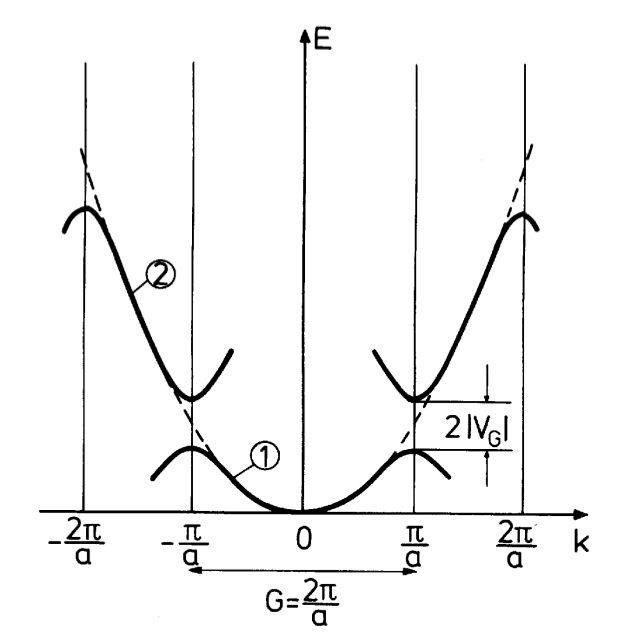
\includegraphics[width=0.5\textwidth]{pics/bloch}
  \end{captionbeside}
  \label{fig:bloch}
\end{figure}

Im Kristall gibt es nun Abweichungen von dem Modell. Zuerst einmal haben Kristalle 
endliche Ausdehnungen, sodass das zuvor als kontinuierlich angenommene 
Energiespektrum diskret ist. Zweitens haben die Elektronen eine Wechselwirkung. 
Diese ist gering im Vergleich zum Potenzial der Kerne, allerdings sorgt sie dafür, 
dass sich die erlaubten Energiewerte für Elektronen eines einzelnen Atoms aufspalten 
in $N$ sehr nahe beieinander liegenden Werten. Für große $N$ sind die erlaubten 
Energiewerte in dem so entstandenen \emph{Band} nahezu kontinuierlich, 
siehe Abb.~\ref{fig:baender1}. Pro Band können  
sich nach dem Pauliprinzip und unter Berücksichtigung des Spins maximal 2N Elektronen 
befinden. Geht die Temperatur gegen Null, so sind die Elektronen in der Konfiguration 
mit der niedrigsten möglichen Gesamtenergie angeordnet. Das oberste dann voll mit 
Elektronen besetzte Band wird als \emph{Valenzband} bezeichnet. Wird die Temperatur 
erhöht, so steht thermische Energie zu Verfügung. Die maximal Energie, die Elektronen 
im Mittel erhalten würden, wenn erlaubte Energiezustände vorhanden wären, wird als 
\emph{Fermienergie} bezeichnet. 
Liegt das Energieband über dem Valenzband unterhalb der Fermienergie oder hat sogar 
einen Überlapp mit dem Valenzband, so können Elektronen Enrgie aufnehmen und in dieses 
Band gelangen. Dort sind sie räumlich deutlich schwächer gebunden und können bei einem 
von außen angelegtem Feld in Richtung des Feldes driften. Daher wird das Band über dem 
Valenzband als \emph{Leitungsband} bezeichnet. Metalle sind deshalb elektrische Leiter, weil 
bei ihnen Leitungs- und Valenzband überlappen. Für das einwertige Natrium ist beispielsweise 
das oberste besetzte Band, das sich aus den 3$s$-Orbitalen zusammensetzt, nur halb besetzt. 
Für zweiwertige Metalle wie Magnesium überlappen sich Leitungs- und Valenzband. 
Bei Isolatoren liegt die Fermienergie niedriger als die untere Kante des Leitungsbandes. 
Die Elektronen können keine Energie eines angelegten Feldes aufnehmen und es kann kein 
Strom fließen. Bei Halbleitern ist die Fermienergie ab einer bestimmten Energie höher 
als die niedrigste Energie des Leitungsbandes. Daher ist ihre Leitfähigkeit 
temperaturabhängig. Siehe Abb.~\ref{fig:baender2}.\cite{demtroder2000experimentalphysik}\\ 

\newcommand{\picwidththeo}{0.48\textwidth}

\begin{figure}
    \centering
    \begin{subfigure}[b]{\picwidththeo}
        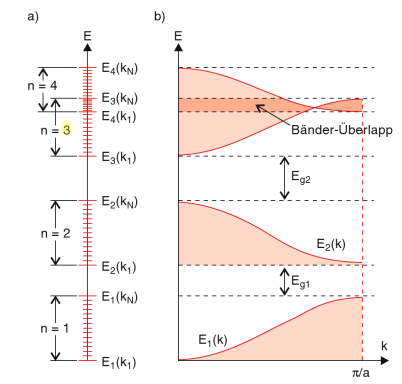
\includegraphics[width=\textwidth]{pics/baender1}
        \caption{Zur Entstehung der Energiebänder. Dargestellt ist die Aufspaltung der erlaubten 
Energiewerte von $N$ Elektronen im Kristall. 
(a) Eindimensionale Darstellung, 
(b) Darstellung von $E_n(k)$, die gestrichelte Linie ist die Grenze der 1. Brillouin-Zone;
aus \cite{demtroder2000experimentalphysik}}
        \label{fig:baender1}
    \end{subfigure}\qquad
    \begin{subfigure}[b]{\picwidththeo}
        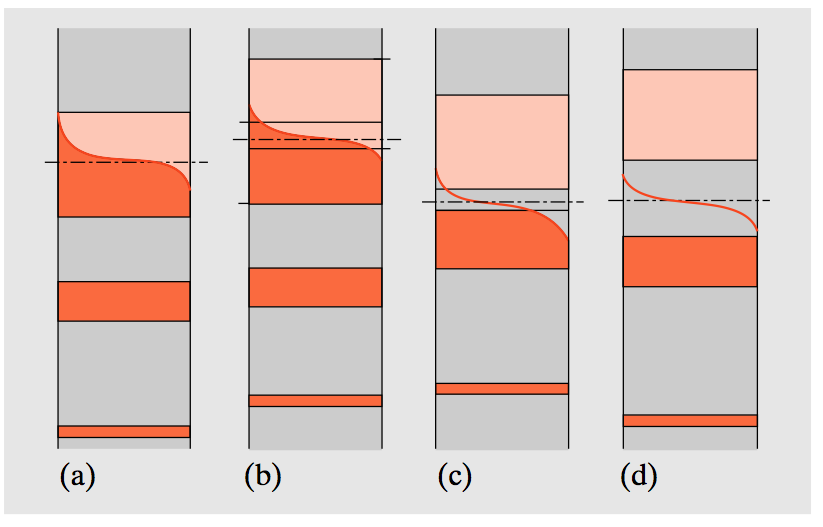
\includegraphics[width=\textwidth]{pics/baender2}
        \caption{Vereinfachte Darstellung des Bändermodells für 
(a) Metalle der ersten Hauptgruppe (Alkalimetalle), 
(b) Metalle der zweitern Hauptgruppe (Erdalkalimetalle), 
(c) Halbleiter (im leitfähigen Zustand)
(d) Isolatoren
aus \cite{vogel1997gerthsen}}
        \label{fig:baender2}
    \end{subfigure}
    \caption{Schemata zum Bändermodell}
    \label{fig:baender}
\end{figure}
